\documentclass[11pt,a4paper]{article}
%%% Preamble %%%

% Packages: I comment ones I don't need or am not using to cut down on compiling time.

	% Default: AMS maths packages

		\usepackage{amsmath}
		\usepackage{amssymb}
		\usepackage{amsfonts}
		\usepackage{mathtools} % Fixes bugs with the ams packages and provides additional functionality.
		
	% Geometry: The layout of the document.

		\usepackage[width = 15 cm, left = 3 cm, height = 23 cm, top = 3 cm]{geometry} % A4 Paper, W = 21 cm, H = 29.7 cm. Paper width = left + width + right, Paper length = top + height + bottom.

	% 	\usepackage{multicol} % Used to switch to two column mode.
	% 	\setlength{\columnsep}{0.75cm} % Determines the length between columns

	% Graphics: Allows images.

		\usepackage{graphicx} % Used to include images.
	% 	\usepackage{float} % For figures in multicolumn
	% 	\usepackage{wrapfig} % Used to have multiple figures in a single beamer slide.

		\graphicspath{./Figures/} % The location of figures used in this document. Trailing / required.

	% Diagrams: Diagram creation.

		\usepackage{tikz} % Creates diagrams, needs calc for arithmetic.
		\usepackage{calc}

	% Figures: Extends figure functionality, allows multiple figures per float environment.

		\usepackage[singlelinecheck=off]{caption} % Needed for subcaption. Adds functionality to all captions. Single line check option needed to left align long table captions.
	%	\usepackage{subcaption} % Allows creation of subfigures, which allows multiple labelled figures per environment.

	% Tables: Extends table functionality, allows multiple page tables.

		\usepackage{booktabs} % Enhances tables with additional functionality.
		\usepackage{longtable} % Allows tables to extend to more than one page.
		\usepackage{multirow} % Allows cells to stretch over multiple rows like multicolumn.

	% Titles: Modifies titles, especially for multicolumns

	% 	\usepackage{titlesec}

	% 	\titleformat{\section}
	% 		{\normalfont\Large\bfseries\centering}
	% 		{\thesection}{1ex}{}

	% 	\titleformat{\subsection}
	% 		{\normalfont\large\bfseries\centering}
	% 		{\thesubsection}{1ex}{}

	% Theorems: Defines theorems, axioms, definitions, etc in a custom environment.

	%\usepackage{amsthm} % Needed for the definitions

	%	%This style is in italics and can be used as a subsection
	%	\newtheoremstyle{conditionStyle}% Name
	%		{3pt}% Space above
	%		{3pt}% Space below
	%		{}% Body font
	%		{\parindent}% Indent amount
	%		{\itshape}% Theorem ead font
	%		{:}% Punctuation after theorem ead
	%		{.5em}% Space after theorem ead
	%		{}% Theorem head spec (can be left empty, meaning `normal')

	%	\newtheoremstyle{solutionStyle}% name of the style to be used
	%		{3pt}% measure of space to leave above the theorem. E.g.: 3pt
	%		{3pt}% measure of space to leave below the theorem. E.g.: 3pt
	%		{}% name of font to use in the body of the theorem
	%		{}% measure of space to indent
	%		{\bfseries}% name of head font
	%		{:}% punctuation between head and body
	%		{.5em}% space after theorem head; " " = normal interword space
	%		{}% Manually specify head

	%	\newtheorem{axiom}{Axiom}
	%	\newtheorem{property}{Property}
	%	\newtheorem{rl}{Rule}
	%	\newtheorem{law}{Law}		
	%	\newtheorem{thm}{Theorem}
	%	\newtheorem{ex}{Example}
	%	\newtheorem{prn}{Principle}
	%	\newtheorem{prf}{Proof}
	%	\newtheorem{lma}{Lemma}

	%	\theoremstyle{definition}
	%	\newtheorem{exc}{Excercise}
	%	\newtheorem{defn}{Definition}
	%	\newtheorem{clm}{Claim}

	%	\newtheorem{qst1}{Question}
	%	\newtheorem{qst}{Question}[qst1]
	%	\newtheorem{sol1}{Solution}
	%	\newtheorem{sol}{Solution}[sol1]

	%	\theoremstyle{conditionStyle}
	%	\newtheorem{condition}{Condition}[rl]

	% Utility: Packages that add extra functionality.

	% 	\usepackage{xcolor} % Used to make footnote numbering red.
	% 	\usepackage{esdiff} %easy differentials eg. \diff[n]{y}{x}, \diffp[n]{y}{x}.
		\usepackage{verbatim} % Used to write code.
	%	\usepackage{textcomp} % Provides roman greek letters.
	% 	\usepackage{eurosym} % Provides accurate euro symbol.
	% 	\usepackage{enumerate} % Needed for lists that use lower case roman numerals.
		\usepackage{xfrac} % used for inline fractions (e.g. a/b via \sfrac{a}{b}).
		\usepackage{thmtools}

	% Editing: Packages and settings used to make papers easier to edit and to test output.

	%	\usepackage{lipsum} % Generates Lorem Ipsum.
	%	\usepackage[pagewise]{lineno} % Used for editing to add line numbers to the left hand side. Use \linenumbers to beging and \nolinenumbers to turn off.

	%	\linespread{1.6} % This changes the the line spacing. A line spacing factor of 1.3 is equivalent to one and a half line spacing and 1.6 is equal to double line spacing.

	% Datetime: Changes the date.

		\usepackage[UKenglish]{isodate}% Used to change the date format.
		\cleanlookdateon % Removes the ordinal suffix

	% Custom accents

	% \usepackage{accents}
	
	% \newlength{\dtildeheight}
	% \newcommand{\doubletilde}[1]{%
	%     \settoheight{\dtildeheight}{\ensuremath{\tilde{#1}}}%
	%     \addtolength{\dtildeheight}{-0.35ex}%
	%     \tilde{\vphantom{\rule{1pt}{\dtildeheight}}%
	%     \smash{\tilde{#1}}}}

	% BibLaTeX: The citestyles and bib file used in citations are edited here.

		\usepackage[backend=biber,citestyle=numeric-comp,doi=true,url=true]{biblatex} % Additional functionality for bibtex, use sorting=none to order in terms of appearance rather than alphabetically.
		\addbibresource{Bibliography.bib}

		\usepackage[utf8]{inputenc} % Allows unicode, so that umlauts will appear in the bibliography

	% Microtyping: The microtype package has several options that affect the way the document is compiled, these go here.

		\usepackage[final,tracking=true,kerning=true,spacing=true]{microtype}
		\microtypecontext{spacing=nonfrench}

	% Referencing: All the referencing packages tend to be loaded last to avoid problems. Order is hyperref then cleveref.

		\usepackage[colorlinks=false,pdfborder={0 0 0},citecolor=blue,urlcolor=blue]{hyperref} % Makes all labels hyperlinks, minus the ugly border.
		\usepackage[noabbrev]{cleveref} % Cleveref has made all the time I spent making reference completions redundant, thanks cleveref.

% Command Creation: I comment out the ones I don't need, but keep them as templates for future commands.

	% \renewcommand\thefootnote{\textcolor{red}{\arabic{footnote}}} % Will make the indecies used in footnotes red to keep in line with the documents colour scheme.

	% \newcommand{\degrees}{\, ^{\circ}\mathrm{C}}

	% For tables in multicolumn.

	% \makeatletter
	% 	\newenvironment{tableplease}
	% 	  {\def\@captype{table}}
	% 	  {}
 	%  	\makeatother

 	%  	For centering tables in multicolumn, eliminates unwanted vertical space.

	% \newenvironment{tightcenter}{%
	%  \setlength\topsep{0pt}
	%  \setlength\parskip{0pt}
	%  \begin{center}
	% }{%
	%  \end{center}
	% }

	% Custom Counter Numbering

	% \numberwithin{equation}{qsol} % Equation numbers will follow the numbering scheme of qsol.

% Math operators declaration

	\DeclareMathOperator\erf{erf}

	\usepackage[parfill]{parskip}

% Title: The title that appears in the report is edited here.

	\title{\textbf{Random Walks for Modelling Cell Populations} \\ VRES 2013-14}
	\author{\textbf{Morgan Wall} \\ n7532962}
	\date{\today}

%%% Document %%%

\begin{document}

%%% Title %%%

\maketitle

%%% Abstract %%%

% \begin{abstract}

%	\noindent 

% \end{abstract}

%%% Body %%%

\section{Introduction}
	\label{sec:introduction}
	
	This report documents the tasks completed by Morgan Wall as part of his 2013-14 VRES scholarship with Dr. Matthew Simpson. The project covered the use of random walks in simulating cell motility, proliferation, and interaction in a variety of biological contexts. Furthermore, the derivation and analysis of partial differential equations to model equivalent processes was considered.

% end sec:introduction

\section{Simulating Random Walks in 2D}
	\label{sec:simrandin2d}
	
	Random walk models are widely applicable to a variety of engineering contexts. Several models, either analsyed or proposed by Simpson, were researched \cite{simpson2009diffusing,simpson2010cell}. Each model accounted for cell motility and proliferation, which were essential to the various biological processes being considered. The models varied based on the consideration of cell interactions via volume exclusion or by the proliferation mechanism used. The models covered were reproduced using MATLAB and the C programming language in conjunction with Intel's Math Kernel Libraries (MKL).

	\subsection{Methodology}
		\label{sub:methodology}
		
		The methodology applied for simulating cell processes mimics that of Simpson's prior work \cite{simpson2009diffusing,simpson2010cell}. Simpson considered applying a rectangular lattice with nodes positioned equidistantly. As such, agents can assume positions at $(i, j)$, where $i, j \in \mathbb{N}$. Each non-boundary node $(i, j)$ therefore has the neighbouring nodes: $(i, j + 1)$, $(i, j - 1)$, $(i + 1, j)$, and $(i - 1, j)$. Random walk simulations are conducted on this lattice by intially placing agents at one or more nodes. Typically, a combination of periodic \cite{periodiccond} and reflective boundary conditions \cite{reflectivecond} are imposed on the lattice.

		For discrete cell simulations, random walks involve spatial and temporal parameters. Consequently, time must be discretised into a series of time steps. At the start of a time step, consider the case where there are $N$ agents present. As per Simpson's approach, $N$ agents are selected at random and each selection results in an agent being ``updated''. Depending on the biological process being modelled, an ``update'' can include both motility and proliferation events. A motility event models cell movement and involves generating a random number from a uniform distribution in determining whether an agent attempts to move to an adjacent node. An adjacent node is consequently selected by generating another uniformly distributed random number $S$ and\dots
	
	% end sub:methodology

	\subsection{Implementation}
		\label{sub:implementation}
		
		
	
	% end sub:implementation

	\subsection{Results}
		\label{sub:results}
		
		In modelling a population of agents, Simpson derived partial differential equations by formulating an agent conservation statement for the average occupancy of a lattice site \cite{simpson2009diffusing}. To demonstrate the reproduced model, simulations were conducted and compared against the following initial value problem (IVP):

		\begin{align}
  			\frac{\partial C}{\partial t} &= D \frac{\partial^2 C}{\partial x^2} && -\infty < x < \infty \\ 
  			C(x,0) &= 
  			\begin{cases}
   				0 & x < -h \\
   				C_0 - h & -h < x < h \\
   				0 & x > h
  			\end{cases}
  			&& -\infty < x < \infty
  			\label{eq:ivp_ic}
		\end{align}

		which has the analytic solution
		
		\begin{equation}
			C(x,t) = \frac{C_0}{2} \left(\erf\left(\frac{h - x}{2 \sqrt{Dt}} \right) + \erf\left(\frac{h + x}{2 \sqrt{Dt}} \right)\right).
			\label{eq:analytic_con_prolif}
		\end{equation}
		
		This IVP was derived in \cite{simpson2009diffusing} and is used to describe agent densities for a one-dimensional problem without proliferation. Density data was obtained from the reproduced model by performing simulations on a two-dimensional lattice with periodic boundary conditions and and averaging the occupancy of each column over multiple identically-prepared realisations. As seen in Figure \ref{fig:cell_concentration_1_100}, the reproduced model matches the analytic solution closely as time elapses.

		\begin{figure}[tbh]
			\centering
				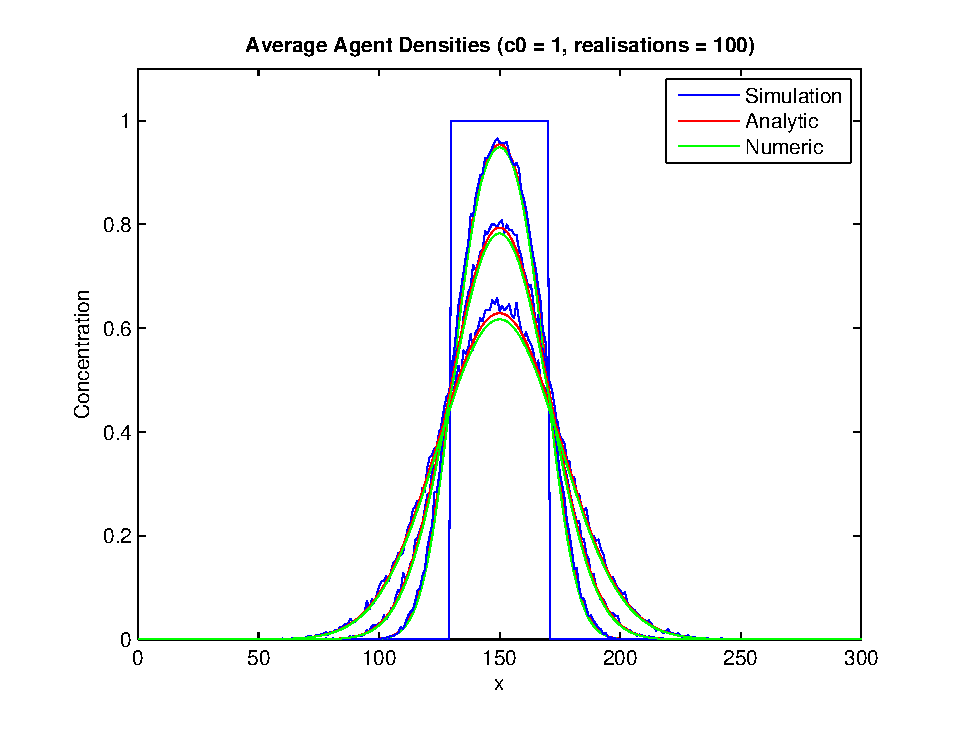
\includegraphics[width=\textwidth]{./Figures/cell_concentration_1_100.eps}
			\caption{Comparison of agent density between the reproduced random walk model and the associated partial differential equation. Density data was obtained by averaging the occupancy of each column over 100 identically-prepared realisations satisfying (\ref{eq:ivp_ic}) where $C_0 = 1$. Densities are given at $t = 0, 200, 500,$ and $1000$ and shows agent density diffusing across the lattice.}
			\label{fig:cell_concentration_1_100}
		\end{figure}

		\subsubsection{Additional Analysis}
			\label{subs:additionalanalysis}
			
			In exploring the various properties of the reproduced model, additional simulations were conducted for differing initial conditions and total realisations performed. As expected from (\ref{eq:analytic_con_prolif}), modifying the initial cell density merely scales the agent density curves (see Figure \ref{fig:cell_concentration_5_100}). Furthermore, as expected by the Law of Large Numbers, the accuracy of the reproduced model was dependent on the number of realisations averaged over \cite{lawlargenum}. As seen between Figures \ref{fig:cell_concentration_1_100} and \ref{fig:cell_concentration_1_10}, an increase in the total realisations performed results in higher accuracy in the final solution.
		
			\begin{figure}[tbh]
				\centering
					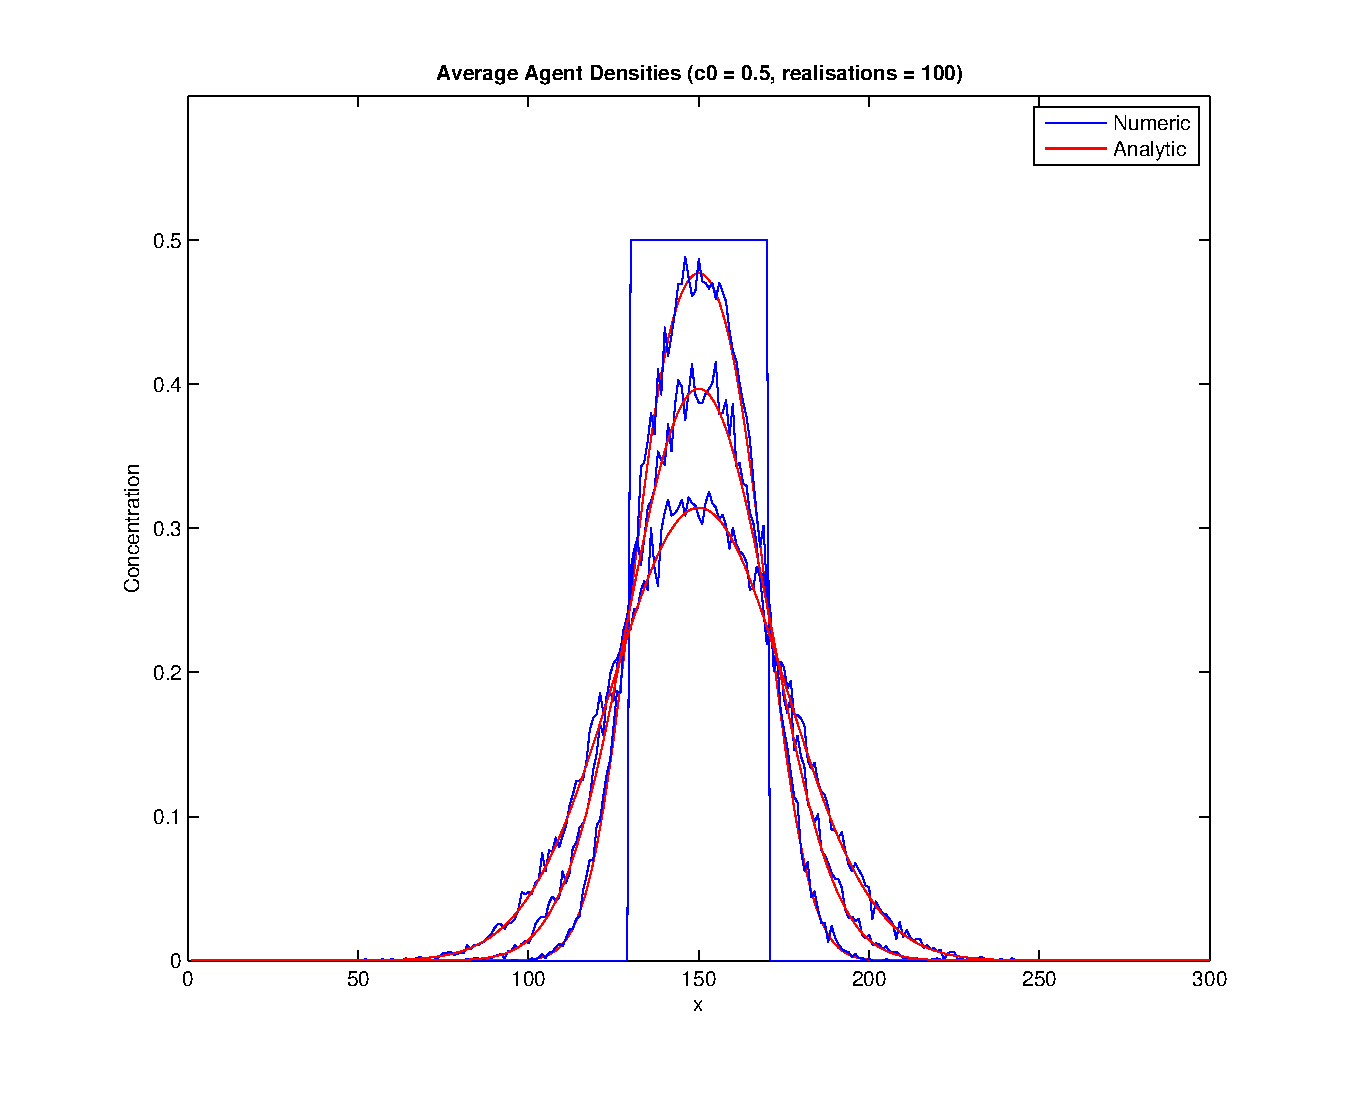
\includegraphics[width=\textwidth]{./Figures/cell_concentration_5_100.eps}
				\caption{Comparison of agent density between the reproduced random walk model and the associated partial differential equation. Density data was obtained by averaging the occupancy of each column over 100 identically-prepared realisations satisfying (\ref{eq:ivp_ic}) where $C_0 = 0.5$. Densities are given at $t = 0, 200, 500,$ and $1000$ and shows agent density diffusing across the lattice.}
				\label{fig:cell_concentration_5_100}
			\end{figure}

			\begin{figure}[tbh]
				\centering
					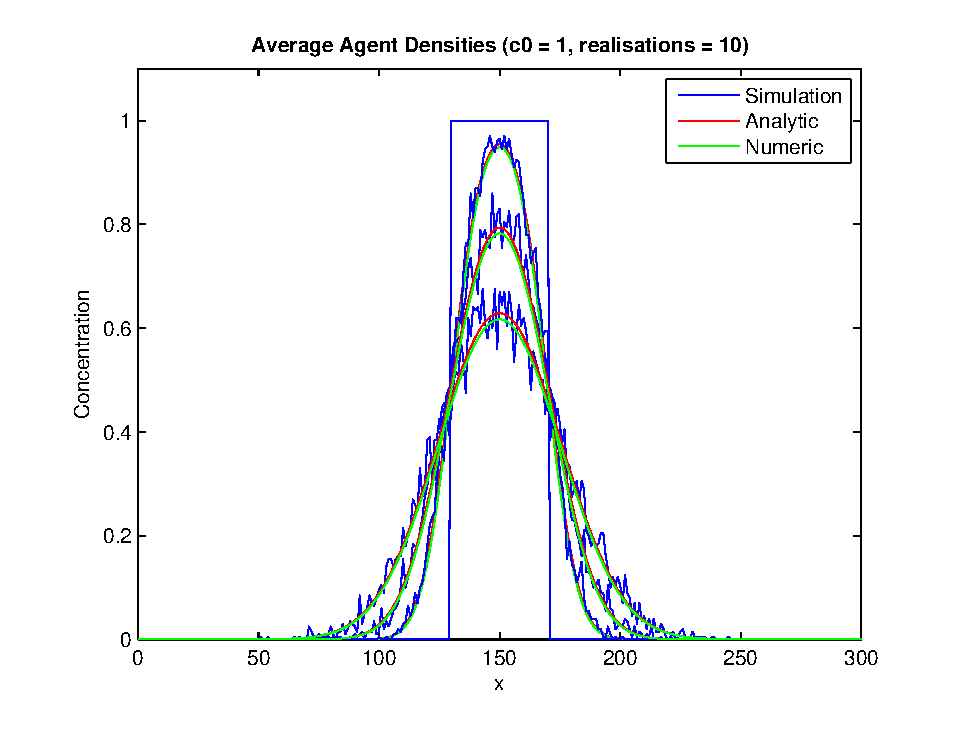
\includegraphics[width=\textwidth]{./Figures/cell_concentration_1_10.eps}
				\caption{Comparison of agent density between the reproduced random walk model and the associated partial differential equation. Density data was obtained by averaging the occupancy of each column over 10 identically-prepared realisations satisfying (\ref{eq:ivp_ic}) where $C_0 = 1$. Densities are given at $t = 0, 200, 500,$ and $1000$ and shows agent density diffusing across the lattice.}
				\label{fig:cell_concentration_1_10}
			\end{figure}

		% end subs:additionalanalysis
	
	% end sub:results

% end sec:simrandin2d

\section{Random Lattices in 1D}
	\label{sec:randlatticein1d}
	
	In simulating cellular phenomena via random walk models, there exists three common methods for handling the spatial domain of interest: equally-spaced lattices, random lattices, and lattice free models. Lattices can be used under a variety of circumstances to discretise the spatial domain into a distinct set of nodes, which cells can consequently occupy. As discussed by Simpson \cite{simpson2010cell}, lattices can be constructed based off the expected size of a cell and the approximate distance they may move over a period of time. In constructing an equally-spaced lattice, nodes are spaced uniformly throughout a domain. Alternatively, nodes are positioned randomly or pseudorandomly within a domain in constructing a random lattice. Unfortunately, cells do not exhibit movement in a rigid, discrete manner, hence lattice-based models may not accurately simulate certain biological processes \cite{plank2013lattice}. Lattice free models avoid this issue by not imposing a spatial discretisation on the simulations, which results in a major performance penalty. 

	Research was conducted into the application of random lattices in simulating cell motility in one dimension. Two approaches were taken in constructing a random lattice: perturbing an equally-spaced lattice and generating node locations pseudorandomly. Under the former, each node position $x_i$ was determined as follows:
	\begin{equation*}
		x_i = y_i + X
	\end{equation*}
	where $y_i$ is the location of the unpertubed node in the equally-spaced lattice and $X$ is a variate sourced from a random distribution. Under the latter, each node position is given by:
	\begin{equation*}
		x_i = Y.
	\end{equation*}
	where $Y$ is a variate sourced from a random distribution. Despite both being random variates, the variance of the distributions from which $\epsilon_i$ and $\gamma_i$ were sourced from varied in comparative simulations. This distinction was established since it was quickly discovered that by imposing large perturbations on an existing lattice, node clustering and impractically large deltas between adjacent nodes can result. Furthermore, random variates were indexed to reflect that pseudorandom numbers are retrieved from streams of values that, as a whole, exhibit properties of a specific statistical distribution. As such, in positioning the $i^{\text{th}}$ node, the $i^{\text{th}}$ value in the relevant stream was sourced. Unless otherwise specified, all random variates are sourced from a uniform distribution. In later simulations, pseudorandom numbers were sourced from a variety of distributions using Intel's Vector Statistical Library (VSL).

	\subsection{Lattice Properties}
		\label{sub:latticeproperties}
		
		Initially, several key characteristics of lattices were identified in determining the preferred method for generating random lattices. The deltas between adjacent nodes and the existence of node clusters were of particular interest in generating physically realistic lattices for simulating cellular phenomenon. A series of random lattices were constructed on a dimensionless 1D region of 20 length units in which 20 nodes would be positioned. For the perturbation method, the equally-spaced lattice consisted of 20 nodes spaced one length unit apart with the first node residing at position zero. 

		Figure \ref{fig:perturbed_layout_1} depicts random lattices generated using the perturbation approach given
		\begin{equation}
			\label{eq:epsilon_dist}
			\epsilon_i \sim \text{Uniform}(-\Delta x, \Delta x)
		\end{equation}
		where $\Delta x$ is the maximum absolute perturbation allowed. These results quickly revealed that large perturbations are detrimental to the construction of random lattices since node clustering is evident. For example, consider the lattices where $\Delta x = 0.1$ and $\Delta x = 0.5$. The former closely resembles an equally-spaced lattice whereas the latter exhibits node clustering around $x = 6$ and $x = 13$ and large unoccupied regions around $x = 5$. Such disparity in lattice spacing can result in erroneous simulations as cell motility can be subject to large variations in distance travelled per unit time. These findings are exacerbated as $\Delta x$ is increased further and is can be shown mathematically by considering the expected value and variance of adjacent node deltas.

		\begin{figure}[tbh]
			\centering
				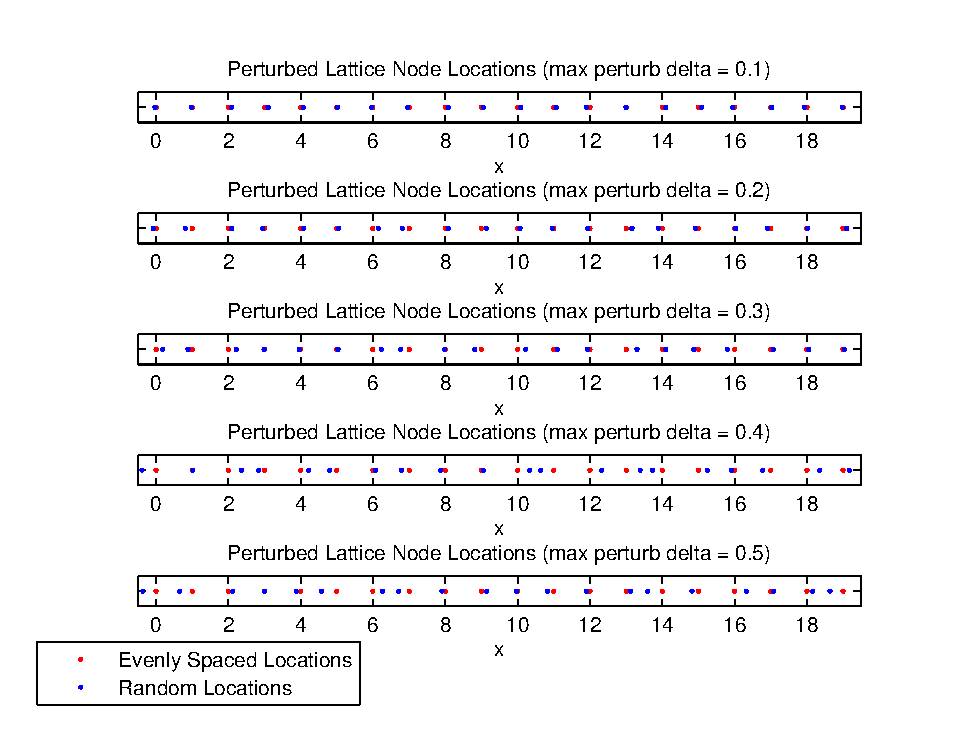
\includegraphics[width=\textwidth]{/Figures/perturbed_layout_1.eps}
			\caption{ }
			\label{fig:perturbed_layout_1}
		\end{figure}

		Consider a random lattice generated using the perturbing approach, where $x_i$ is the position of the $i^\text{th}$ node. Given the unperturbed lattice had a fixed node spacing $\Delta x$ the expected node spacing is given by
		\begin{align*}
			\mathrm{E} \left(x_i - x_{i-1} \right) &= \mathrm{E} \left(y_i + \epsilon_i - y_{i-1} - \epsilon_{i-1} \right) \\
			&= \mathrm{E} \left(\Delta x + \epsilon_i - \epsilon_{i-1} \right).
		\end{align*}
		For generality, assume $\epsilon_i$ and $\epsilon_{i-1}$ are continous random variables with probably density functions $f(\alpha)$ and $g(\beta)$, respectively, then
		\begin{align*}
			\phantom{\mathrm{E} \left(x_i - x_{i-1} \right)}
			&\begin{aligned}
				\mathllap{\mathrm{E} \left(x_i - x_{i-1} \right)} &= \int_{-\infty}^{\infty} \int_{-\infty}^{\infty} \left (\Delta x + \alpha - \beta\right) f(\alpha) g(\beta) \,\mathrm{d}\alpha \, \mathrm{d}\beta
			\end{aligned} \\
			&\begin{aligned}
				&= \Delta x \int_{-\infty}^{\infty} \int_{-\infty}^{\infty} f(\alpha) g(\beta) \,\mathrm{d}\alpha \, \mathrm{d}\beta \\
					&\qquad + \int_{-\infty}^{\infty} \int_{-\infty}^{\infty} \alpha f(\alpha) g(\beta) \,\mathrm{d}\alpha \, \mathrm{d}\beta \\
						&\qquad\qquad - \int_{-\infty}^{\infty} \int_{-\infty}^{\infty} \beta f(\alpha) g(\beta) \,\mathrm{d}\alpha \, \mathrm{d}\beta
			\end{aligned} \\
			&\begin{aligned}
				&= \Delta x + \int_{-\infty}^{\infty} g(\beta) \, \mathrm{d}\beta \int_{-\infty}^{\infty} \alpha f(\alpha) \,\mathrm{d}\alpha \\
					&\qquad - \int_{-\infty}^{\infty} f(\alpha) \,\mathrm{d}\alpha \int_{-\infty}^{\infty} \beta g(\beta) \,\mathrm{d}\beta
			\end{aligned} \\
			&= \Delta x + \mathrm{E} \left(\epsilon_i \right) - \mathrm{E} \left(\epsilon_{i-1} \right).
		\end{align*}
		Hence, if $\epsilon_i$ and $\epsilon_{i-1}$ are independent and identically distributed continuous random variables, then
		\begin{equation*}
			\mathrm{E} \left(x_i - x_{i-1} \right) = \Delta x.
		\end{equation*}
		As such, if we were to investigate the average delta between adjacent nodes over many meshes, for example, then by the Law of Large Numbers, the expected delta is that of the equally-spaced lattice. This finding presupposes the expected value of $\epsilon_i$ is zero. In this case, this finding does not describe the existence of node clustering and large deltas between nodes as seen previously. Instead, consider finding the variance of the same statistic as follows:
		\begin{align*}
			\mathrm{Var} \left(x_i - x_{i-1} \right) &= \mathrm{Var} \left(y_i + \epsilon_i - y_{i-1} - \epsilon_{i-1} \right) \\
			&= \mathrm{Var} \left(\Delta x + \epsilon_i - \epsilon_{i-1} \right).
		\end{align*}
		Making the same generality assumption for $\epsilon_i$ and $\epsilon_{i-1}$ as before and letting $\Gamma = \Delta x + \epsilon_i - \epsilon_{i-1}$ be a continous random variable gives
		\begin{equation*}
			\mathrm{Var} \left(x_i - x_{i-1} \right) = \mathrm{Var} \left(\Gamma \right) = \int_{-\infty}^{\infty} \left(\gamma - \mathrm{E}(\Gamma) \right)^2 \,\mathrm{d}\gamma
		\end{equation*}
		where
		\begin{equation*}
			\mathrm{E} \left(\Gamma \right) = \Delta x + \mathrm{E} \left(\epsilon_{i} \right) - \mathrm{E} \left(\epsilon_{i-1} \right).
		\end{equation*}
		Considering the case where $\epsilon_i$ and $\epsilon_{i-1}$ are independent and identitically distributed continuous random variables, then
		\begin{align*}
			\phantom{\mathrm{Var} \left(x_i - x_{i-1} \right)}
			&\begin{aligned}
				\mathllap{\mathrm{Var} \left(x_i - x_{i-1} \right)} &= \int_{-\infty}^{\infty} \left(\gamma - \Delta x \right)^2 \,\mathrm{d}\gamma \\
			\end{aligned} \\
			&\begin{aligned}
				&= \int_{-\infty}^{\infty} \int_{-\infty}^{\infty} \left(\gamma - \Delta x \right)^2 \,\mathrm{d}\gamma
			\end{aligned}
		\end{align*}
	
	% end sub:latticeproperties

	\subsection{Simulating Random Walks}
		\label{sub:simulatingrandomwalks}
		
		\subsubsection{Net Agent Displacement}
			\label{subs:netagentdisplacement}
			
			
		
		% end subs:netagentdisplacement
	
	% end sub:simulatingrandomwalks 

% end sec:randlatticein1d

\section{Investigating Travelling Wave Solutions}
	\label{sec:investigatingfishersequation}
	
	\subsection{Phase Plane Analysis of Fisher's Equation}
		\label{sub:phaseplaneanalysisoffishersequation}
		
		As part of modelling cell invasion fronts, travelling wave solutions of partial differential equations was researched. The travelling wave solutions of Fisher's equation for population growth,
		\begin{equation}
			 \label{eq:fisherseq}
			 \frac{\partial U}{\partial t} = \nu \frac{\partial^2 U}{\partial y^2} + k U (1 - U),
		\end{equation}
		was thoroughly analysed via \cite{canosa1973nonlinear}. To ease subsequent analysis, (\ref{eq:fisherseq}) can be nondimensionalised via the unit-reducing substitutions:
		\begin{align}
			 \label{eq:timeSubFisher}
			 \tau &= \alpha t \qquad \text{and} \\
			 \label{eq:spaceSubFisher} 
			 x &= \beta y
		\end{align}
		where $\alpha$ and $\beta$ have units $t^{-1}$ and $m^{-1}$, respectively. Applying the substitution in (\ref{eq:timeSubFisher}) and the chain rule, we obtain:
		\begin{align*}
			 \frac{\partial U}{\partial \tau} \frac{d \tau}{d t} &= \nu \frac{\partial^2 U}{\partial y^2} + k U (1 - U) \\ 
			 \alpha \frac{\partial U}{\partial \tau} &= \nu \frac{\partial^2 U}{\partial y^2} + k U (1 - U)
		\end{align*}
		By inspection, it is clear that (\ref{eq:fisherseq}) can be nondimensionalised in time and simplified when $\alpha = k$. Hence,
		\begin{equation}
			 \label{eq:timeSubbedFisher}
			 \frac{\partial U}{\partial \tau} = \frac{\nu}{k} \frac{\partial^2 U}{\partial y^2} + U (1 - U)
		\end{equation}
		Applying (\ref{eq:spaceSubFisher}) in a similar manner gives
		\begin{equation*}
			 \frac{\partial U}{\partial \tau} = \frac{\beta^2 \nu}{k} \frac{\partial^2 U}{\partial x^2} + U (1 - U).
		\end{equation*}
		As such, (\ref{eq:timeSubbedFisher}) can be nondimensionalised in space and simplified when $\beta = \sqrt{\sfrac{k}{\nu}}$, which results in
		\begin{equation}
			 \label{eq:timeSpaceSubbedFisher}
			 \frac{\partial U}{\partial \tau} = \frac{\partial^2 U}{\partial x^2} + U (1 - U).
		\end{equation}
		As discussed by Canosa \cite{canosa1973nonlinear}, this nondimensionalised equation describes nonlinear population growth in one spatial dimension. Consequently, the modelled habitat (i.e. space) can only feasibly support a maximum population per unit length. Given the form of the logistic source term in (\ref{eq:timeSpaceSubbedFisher}), suppose that maximum population is unity. The following initial condition can therefore be applied:
		\begin{equation}
			 \label{eq:fisherInitialCondition}
			 0 \le U(x, 0) \le 1, \qquad -\infty < x < \infty.
		\end{equation}
		Canosa \cite{canosa1973nonlinear} was specifically interested solving (\ref{eq:timeSpaceSubbedFisher}) subject to (\ref{eq:fisherInitialCondition}) such that all the derivatives in $x$ tended to zero as $x \to \pm \infty$ coupled with the following far-field conditions:
		\begin{equation}
			 \label{eq:fisherBoundaryCondition}
			 \lim_{x\to -\infty} U(x,\tau) = 1 \qquad \lim_{x\to \infty} U(x,\tau) = 0 \qquad t \ge 0.
		\end{equation}
		Any one-dimensional partial differential equations in space and time, $U(x,\tau)$, exhibiting travelling wave solutions supports the transformation
		\begin{equation}
			 \label{eq:travellingWaveSub}
			 U(x,t) = U(x - c\tau) \equiv U(s)
		\end{equation}
		which merges both time and space variables to provide a ``standing wave'' solution where the spatial origin is locked at the peak of the travelling wave moving at speed $c$. As such, the spatial coordinate system can be seen to translate in time in moving with the peak of the wave. Applying (\ref{eq:travellingWaveSub}) with the chain rule gives
		\begin{equation*}
			 -c \frac{d U}{d s} = \frac{d^2 U}{d s^2} + U(1 - U)
		\end{equation*}
		which has reduced Fisher's equation into a second order non-linear partial differential equation. This equation can be further simplified into the following system of first order differential equations
		\begin{align}
			 \label{eq:fisherDESystemU}
			 \frac{d U}{d s} &= V(s) \\
			 \label{eq:fisherDESystemV}
			 \frac{d V}{d s} &= U^2 - U - cV.
		\end{align}
		Phase plane analysis was conducted on (\ref{eq:fisherDESystemU}) and (\ref{eq:fisherDESystemV}) using pplane8 for MATLAB \cite{pplane8}. 
		
		Fisher originally discovered that (\ref{eq:fisherseq}) has travelling wave solutions where $c \ge 2$. This fact can be verified by solving the eigenvalue problem associated with (\ref{eq:fisherDESystemU}) and (\ref{eq:fisherDESystemV}) to determine the nature of any critical points in the phase plane. Given $c \ge 2$ it can be shown that, $(U, V) = (0, 0)$ is a stable node and $(U, V) = (1, 0)$ is a saddle point. Conversely, given $c < 2$, $(U, V) = (0, 0)$ is a stable spiral. The phase planes seen in Figures \ref{fig:canosa_invalid} and \ref{fig:canosa_valid} illustrate these results for specific values of $c$. Figure \ref{fig:canosa_invalid} exhibits the physically impossible solutions for $c < 2$ as discussed by Canosa \cite{canosa1973nonlinear}. Note how certain phase trajectories can lead to negative values of $U$, which is physically impractical in modelling population growth.

		\begin{figure}[tbh]
			\centering
				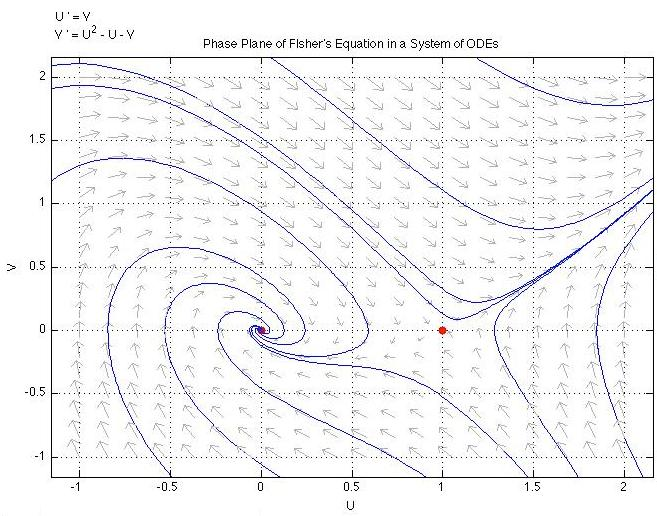
\includegraphics[width=\textwidth]{/Figures/canosa_invalid.jpeg}
			\caption{\slshape }
			\label{fig:canosa_invalid}
		\end{figure}

		\begin{figure}[tbh]
			\centering
				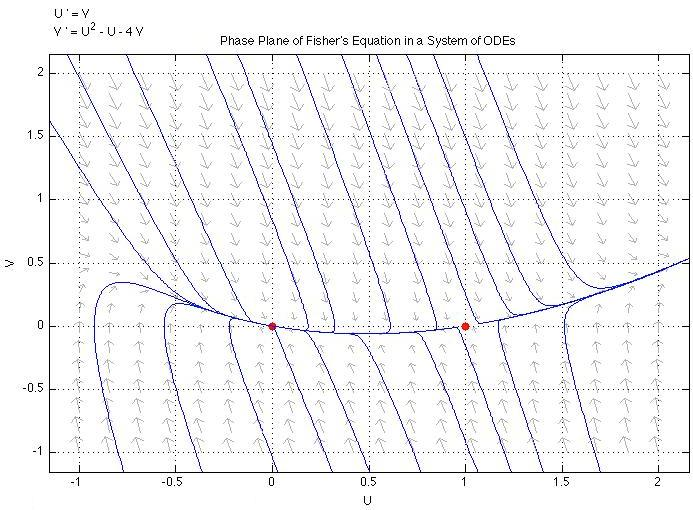
\includegraphics[width=\textwidth]{/Figures/canosa_valid.jpeg}
			\caption{\slshape }
			\label{fig:canosa_valid}
		\end{figure}

	% end sub:phaseplaneanalysisoffishersequation

	\subsection{Solving Fisher's Equation}
		\label{sub:solvingfishersequation}
		
		In order to better understand the travelling wave solutions to Fisher's equation, the following IBVP was solved numerically using MATLAB's pdepe function:
		\begin{align*}
			 \label{eq:fisherNumericIBVP}
			 \frac{\partial U}{\partial \tau} &= \frac{\partial^2 U}{\partial x^2} + U(1 - U) && 0 \le x \le 100 && t \ge 0 \\
			 U(0, \tau) &= 1 && \tau \ge 0 \\
			 U(100, \tau) &= 0 && \tau \ge 0 \\
			 U(x, 0) &= 
			 \begin{cases}
   				1 & x \le 50 \\
   				0 & \text{otherwise}
  			\end{cases}
  			&& 0 \le x \le 100.
		\end{align*}
		The solutions, for varying timesteps, can be seen in Figure \ref{fig:fishers_equation_sol_pdepe}. From the figure it is clear that a static wavefront is formed which moves throughout space at a constant speed. This wavefront does not hold at the boundaries in order to satisfy the conditions imposed there. As a side note, the solutions did exhibit monotonicity issues. After discussion with Simpson, it was determined that this is due to MATLAB's pdepe function using the method of lines, which can result in physically unrealistic solutions. It was decided that alternative means for solving Fisher's equation would be pursued as a result. 

		Solutions to Fisher's equation were investigated for various initial conditions to observe how the logistic source term reacts to overpopulated and underpopulated regions. As expected, provided $U \ge 0$, the solutions continue to form a travelling wavefront. This is due to the logistic source term compensating for regions which do not satisfy the carrying capacity of unity. Likewise, in the event that $U < 0$, the solutions diverge to $-\infty$. It is clear that the logistic source term plays an integral role in forming travelling wave solutions of a specific amplitude.

		\begin{figure}[tbh]
			\centering
				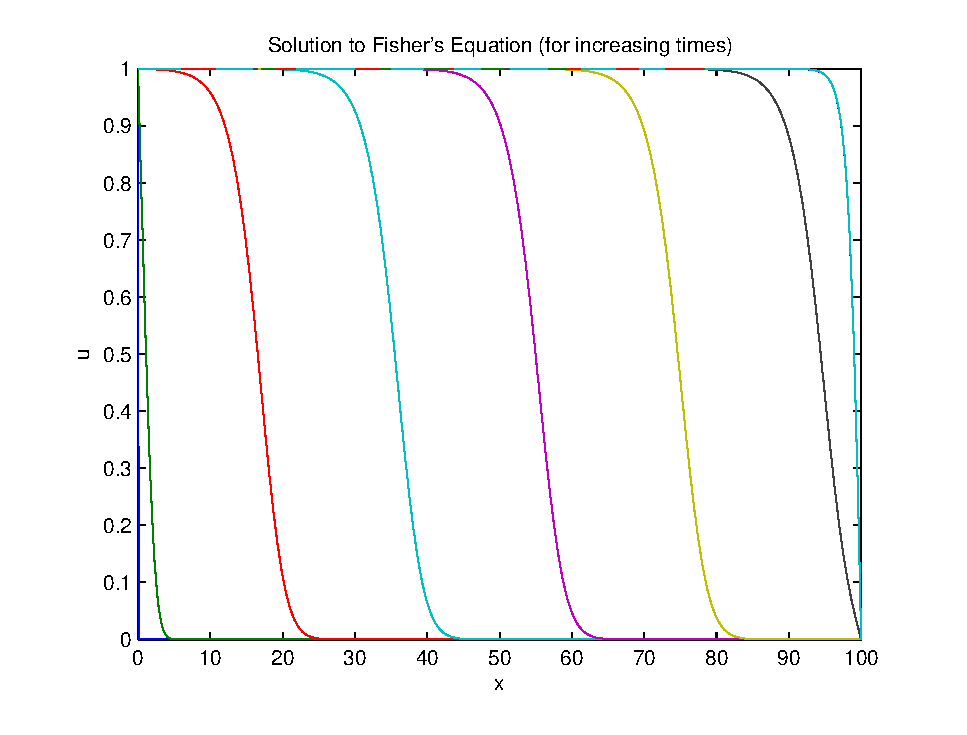
\includegraphics[width=\textwidth]{/Figures/fishers_equation.eps}
			\caption{[insert figure description]}
			\label{fig:fishers_equation_sol_pdepe}
		\end{figure}
	
	% end sub:solvingfishersequation

% end sec:investigatingfishersequation

%%% Bibliography %%%

\clearpage
\printbibliography

\end{document}
